\documentclass[conference]{IEEEtran}
\IEEEoverridecommandlockouts
% The preceding line is only needed to identify funding in the first footnote. If that is unneeded, please comment it out.
\usepackage{cite}
\usepackage{amsmath,amssymb,amsfonts}
\usepackage{algorithmic}
\usepackage{graphicx}
\usepackage{textcomp}
\usepackage{xcolor}
\usepackage{listings}
\usepackage{hyperref}
\usepackage{xparse}


\definecolor{mGreen}{rgb}{0,0.6,0}
\definecolor{mGray}{rgb}{0.5,0.5,0.5}
\definecolor{mPurple}{rgb}{0.58,0,0.82}
\definecolor{backgroundColour}{rgb}{0.95,0.95,0.92}

\NewDocumentCommand{\codeword}{v}{%
	\texttt{\textcolor{blue}{#1}}%
}

\lstdefinestyle{CStyle}{
	backgroundcolor=\color{backgroundColour},   
	commentstyle=\color{mGreen},
	keywordstyle=\color{magenta},
	numberstyle=\tiny\color{mGray},
	stringstyle=\color{mPurple},
	basicstyle=\footnotesize,
	breakatwhitespace=false,         
	breaklines=true,                 
	captionpos=b,                    
	keepspaces=true,                 
	numbers=left,                    
	numbersep=5pt,                  
	showspaces=false,                
	showstringspaces=false,
	showtabs=false,                  
	tabsize=2,
	language=C
}

\lstset{language=C,keywordstyle={\bfseries \color{blue}}}

\def\BibTeX{{\rm B\kern-.05em{\sc i\kern-.025em b}\kern-.08em
    T\kern-.1667em\lower.7ex\hbox{E}\kern-.125emX}}
\begin{document}

\title{Weather Clock\\
{\footnotesize \textsuperscript{*}Note: Sub-titles are not captured in Xplore and
should not be used}
\thanks{Identify applicable funding agency here. If none, delete this.}
}

\author{\IEEEauthorblockN{1\textsuperscript{st} Imron Gamidli}
\IEEEauthorblockA{\textit{Internationale In} \\
\textit{Hochschule Fulda}\\
Fulda, Deutschland \\
imron.gamidli@lt.hs-fulda.de}
\and
\IEEEauthorblockN{2\textsuperscript{nd} Hussain Ali}
\IEEEauthorblockA{\textit{Internationale In} \\
	\textit{Hochschule Fulda}\\
	Fulda, Deutschland \\
	imron.gamidli@lt.hs-fulda.de}
}

\maketitle

\begin{abstract}

\end{abstract}

\begin{IEEEkeywords}
dht22, arduino, uno, 
\end{IEEEkeywords}

\section{DHT22 Sensor}

\subsection{Beschreibung}
Der DHT22 ist ein einfacher, preiswerter digitaler Temperatur- und Feuchtigkeitssensor. Er verwendet einen kapazitiven Feuchtigkeitssensor und einen Thermistor, um die Umgebungsluft zu messen, und spuckt ein digitales Signal auf dem Datenpin aus (keine analogen Eingangspins erforderlich). Er ist recht einfach zu bedienen, erfordert aber ein sorgfältiges Timing bei der Datenerfassung. Der einzige wirkliche Nachteil dieses Sensors ist, dass man nur alle 2 Sekunden neue Daten von ihm erhalten kann, so dass bei Verwendung unserer Bibliothek die Sensormesswerte bis zu 2 Sekunden alt sein können.

Verbinden Sie einfach den ersten Pin auf der linken Seite mit 3-5V Strom, den zweiten Pin mit Ihrem Dateneingangspin und den ganz rechten Pin mit Masse. Obwohl der Sensor ein einziges Kabel zum Senden von Daten verwendet, ist er nicht mit Dallas One Wire kompatibel! Wenn Sie mehrere Sensoren wünschen, muss jeder seinen eigenen Datenpin haben.

Im Vergleich zum DHT11 ist dieser Sensor präziser, genauer und funktioniert in einem größeren Temperatur-/Feuchtigkeitsbereich, ist aber auch größer und teurer.

Wird mit einem 4.7K - 10K Widerstand geliefert, den Sie als Pullup vom Daten-Pin zu VCC verwenden wollen.

\subsection{Technische Daten}
\begin{itemize}
	\item Geringe Kosten
	\item 3 bis 5V Stromversorgung und E/A
	\item Maximal 2,5 mA Stromverbrauch während der Umwandlung (während der Datenabfrage)
	\item Gut geeignet für 0-100% Luftfeuchtigkeit mit 2-5% Genauigkeit
	\item Gut geeignet für Temperaturmessungen von -40 bis 80°C mit einer Genauigkeit von ±0,5°C
	\item Abtastrate nicht mehr als 0,5 Hz (einmal alle 2 Sekunden)
	\item Gehäusegröße 27mm x 59mm x 13,5mm (1,05" x 2,32" x 0,53")
	\item 4 Stifte, 0,1" Abstand 
	\item Gewicht (nur der DHT22): 2,4g
\end{itemize}

	
\begin{figure}
	\begin{center}
		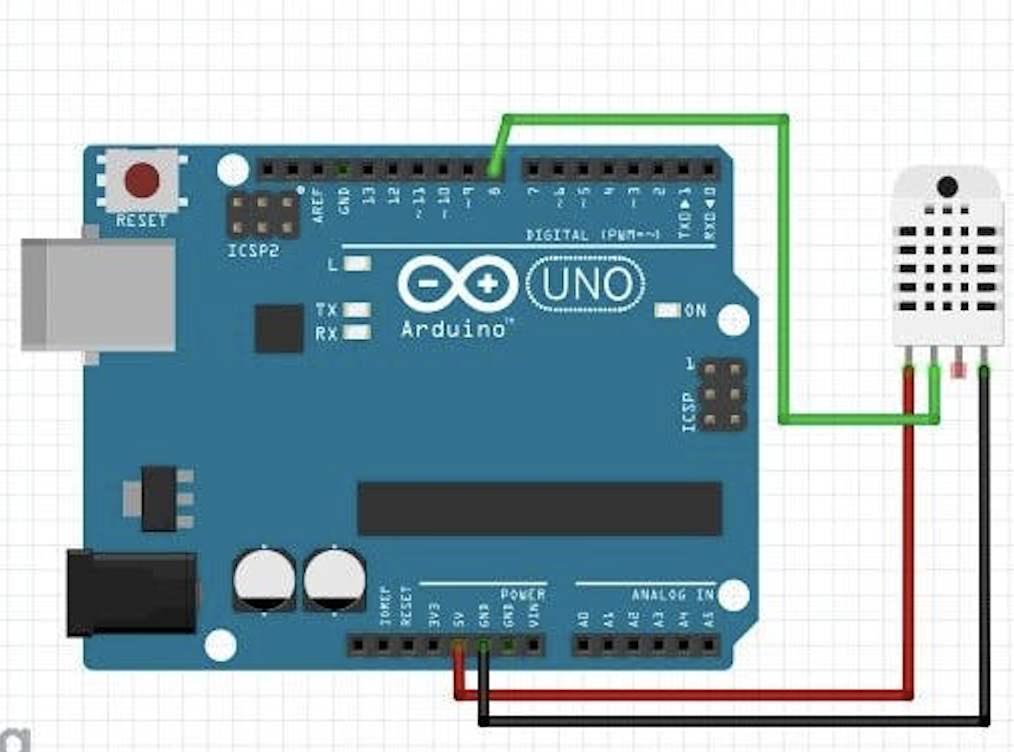
\includegraphics[scale=0.4]{dht22}
	\end{center}
	\caption{DHT22 Sensor}
\end{figure}

Es ist ziemlich einfach, die DHT-Sensoren anzuschließen. Sie haben vier Stifte VCC - roter Draht Schließen Sie an 3,3 - 5V Strom an. Manchmal reicht die 3,3-V-Spannung nicht aus, in diesem Fall versuchen Sie es mit einer 5-V-Spannung. Datenausgang - weißes oder gelbes Kabel Nicht angeschlossen Masse - schwarzes Kabel Ignorieren Sie einfach Pin 3, er wird nicht verwendet. Dieses Diagramm zeigt, wie wir für die Testskizze anschließen werden. Schließen Sie Daten an Pin 2 an, Sie können dies später auf jeden beliebigen Pin ändern.

\subsection{Implementierung im Projekt}
DHT22 war nützlich für unseres Projekt. Mithilfe diesen Sensor, bekommen wir Temperatur und Feuchtigkeit Daten. Damit es möglich wird, Sensordaten zu lesen, bestimmte Bibliothek muss installiert und importiert soll. Die Bibliothek für DHT22 heißt \textit{DHT sensor library} und installiert wurde vom \url{https://github.com/adafruit/DHT-sensor-library} . Nachdem wir die Bibliothek installiert haben, haben wir diese importiert.


\begin{lstlisting}[style=CStyle]
#include <DHT.h>;
\end{lstlisting}

Diese Bibliothek ermöglicht uns eine DHT Instanz initialisieren. Hier man sieht wir haben PIN 13 für DHT Kommunikation. Danach haben wir DHT22 Instanz erstellt.

\begin{lstlisting}[style=CStyle]
#define DHTPIN 13	// what pin we're connected to
#define DHTTYPE DHT22	// DHT 22 
DHT dht(DHTPIN, DHTTYPE);	// Initialize DHT 
\end{lstlisting}

Wir werden später Daten aus dem Sensor in Variablen speichern. Dafür haben wir zwei Variablen, \textsf{hum} für Feuchtigkeit und \textsf{temp} für Temperatur deklariert. 

\begin{lstlisting}[style=CStyle]
float hum;	//Stores humidity value
float temp;	//Stores temperature value
\end{lstlisting}

In \textsf{setup()} Funktion haben wir die DHT Instanz gestartet. Das heißt, die Instanz läuft und wir können jederzeit Feuchtigkeit und Temperaturdaten anfragen. 

\begin{lstlisting}[style=CStyle]
void setup()
{
	dht.begin();
}
\end{lstlisting}

In der Schleife \textsf{loop()} das Programm liest Feuchtigkeitswert mit \textsf{readHumidity()} und speichert in \textsf{hum} variable. Auf die gleiche Weise Temperatur wird mit \textsf{readTemperature()} gelesen und in \textsf{temp} gespeichert. 

\begin{lstlisting}[style=CStyle]
void loop()
{
	//Read data and store it to variables hum and temp
	hum = dht.readHumidity();
	temp = dht.readTemperature();
	
}
\end{lstlisting}

Letzte Aufgabe ist auf dem Display darzustellen, das vorher  mit entsprechender Adresse initialisiert wurde. Wir haben zwei Displays, für DHT Daten haben wir erste Reihe des erstens Display benutzt. 

\begin{lstlisting}[style=CStyle]
	void loop()
	{
		//Read data and store it to variables hum and temp
		hum = dht.readHumidity();
		temp = dht.readTemperature();
		
		lcd1.setCursor(0, 0);
		lcd1.print("tmp:");
		lcd1.print(temp); 
		lcd1.setCursor(6, 0);
		lcd1.print((char)223);
		lcd1.print("C hum:");
		lcd1.print(hum);
		lcd1.setCursor(15, 0);
		lcd1.print("%");
		
	}
\end{lstlisting}


\subsection{Figures and Tables}
\paragraph{Positioning Figures and Tables} Place figures and tables at the top and 
bottom of columns. Avoid placing them in the middle of columns. Large 
figures and tables may span across both columns. Figure captions should be 
below the figures; table heads should appear above the tables. Insert 
figures and tables after they are cited in the text. Use the abbreviation 
``Fig.~\ref{fig}'', even at the beginning of a sentence.

\begin{table}[htbp]
\caption{Table Type Styles}
\begin{center}
\begin{tabular}{|c|c|c|c|}
\hline
\textbf{Table}&\multicolumn{3}{|c|}{\textbf{Table Column Head}} \\
\cline{2-4} 
\textbf{Head} & \textbf{\textit{Table column subhead}}& \textbf{\textit{Subhead}}& \textbf{\textit{Subhead}} \\
\hline
copy& More table copy$^{\mathrm{a}}$& &  \\
\hline
\multicolumn{4}{l}{$^{\mathrm{a}}$Sample of a Table footnote.}
\end{tabular}
\label{tab1}
\end{center}
\end{table}

\begin{figure}[htbp]
\centerline{
\includegraphics{fig1.png}}
\caption{Example of a figure caption.}
\label{fig}
\end{figure}

Figure Labels: Use 8 point Times New Roman for Figure labels. Use words 
rather than symbols or abbreviations when writing Figure axis labels to 
avoid confusing the reader. As an example, write the quantity 
``Magnetization'', or ``Magnetization, M'', not just ``M''. If including 
units in the label, present them within parentheses. Do not label axes only 
with units. In the example, write ``Magnetization (A/m)'' or ``Magnetization 
\{A[m(1)]\}'', not just ``A/m''. Do not label axes with a ratio of 
quantities and units. For example, write ``Temperature (K)'', not 
``Temperature/K''.

\section*{Acknowledgment}

The preferred spelling of the word ``acknowledgment'' in America is without 
an ``e'' after the ``g''. Avoid the stilted expression ``one of us (R. B. 
G.) thanks $\ldots$''. Instead, try ``R. B. G. thanks$\ldots$''. Put sponsor 
acknowledgments in the unnumbered footnote on the first page.

\section*{References}

Please number citations consecutively within brackets \cite{b1}. The 
sentence punctuation follows the bracket \cite{b2}. Refer simply to the reference 
number, as in \cite{b3}---do not use ``Ref. \cite{b3}'' or ``reference \cite{b3}'' except at 
the beginning of a sentence: ``Reference \cite{b3} was the first $\ldots$''

Number footnotes separately in superscripts. Place the actual footnote at 
the bottom of the column in which it was cited. Do not put footnotes in the 
abstract or reference list. Use letters for table footnotes.

Unless there are six authors or more give all authors' names; do not use 
``et al.''. Papers that have not been published, even if they have been 
submitted for publication, should be cited as ``unpublished'' \cite{b4}. Papers 
that have been accepted for publication should be cited as ``in press'' \cite{b5}. 
Capitalize only the first word in a paper title, except for proper nouns and 
element symbols.

For papers published in translation journals, please give the English 
citation first, followed by the original foreign-language citation \cite{b6}.

\begin{thebibliography}{00}
\bibitem{b1} G. Eason, B. Noble, and I. N. Sneddon, ``On certain integrals of Lipschitz-Hankel type involving products of Bessel functions,'' Phil. Trans. Roy. Soc. London, vol. A247, pp. 529--551, April 1955.
\bibitem{b2} J. Clerk Maxwell, A Treatise on Electricity and Magnetism, 3rd ed., vol. 2. Oxford: Clarendon, 1892, pp.68--73.
\bibitem{b3} I. S. Jacobs and C. P. Bean, ``Fine particles, thin films and exchange anisotropy,'' in Magnetism, vol. III, G. T. Rado and H. Suhl, Eds. New York: Academic, 1963, pp. 271--350.
\bibitem{b4} K. Elissa, ``Title of paper if known,'' unpublished.
\bibitem{b5} R. Nicole, ``Title of paper with only first word capitalized,'' J. Name Stand. Abbrev., in press.
\bibitem{b6} Y. Yorozu, M. Hirano, K. Oka, and Y. Tagawa, ``Electron spectroscopy studies on magneto-optical media and plastic substrate interface,'' IEEE Transl. J. Magn. Japan, vol. 2, pp. 740--741, August 1987 [Digests 9th Annual Conf. Magnetics Japan, p. 301, 1982].
\bibitem{b7} M. Young, The Technical Writer's Handbook. Mill Valley, CA: University Science, 1989.
\end{thebibliography}
\vspace{12pt}
\color{red}
IEEE conference templates contain guidance text for composing and formatting conference papers. Please ensure that all template text is removed from your conference paper prior to submission to the conference. Failure to remove the template text from your paper may result in your paper not being published.

\end{document}
